

\begin{frame}{Providing Context}

 \begin{center}
  \fbox{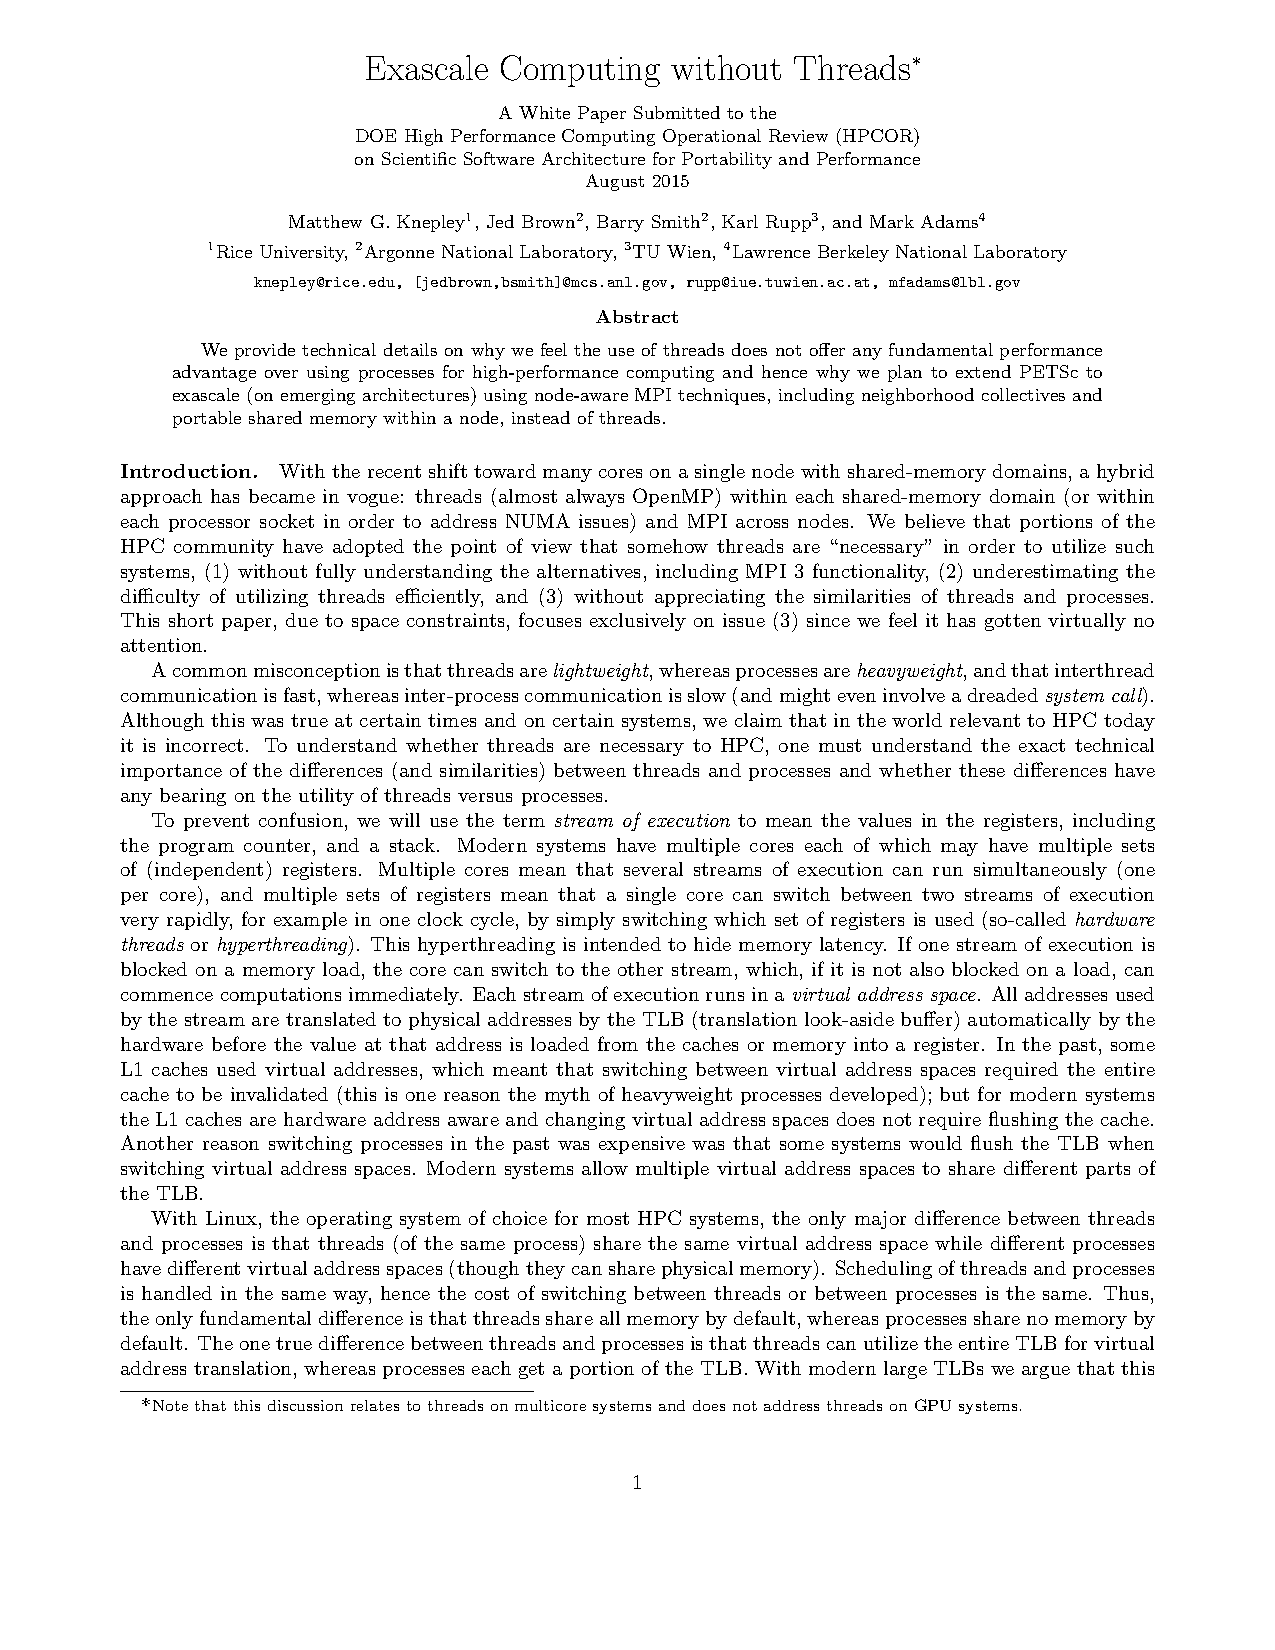
\includegraphics[clip,trim=0.5cm 20.5cm 0.5cm 0.4cm,width=0.75\textwidth]{figures/exascale-without-threads.pdf}} \\
  {\scriptsize \texttt{https://www.orau.gov/hpcor2015/whitepapers/Exascale\_Computing\_without\_Threads-Barry\_Smith.pdf}}
 \end{center}

 \begin{block}{PETSc Developers Care About Recent Developments}
  \begin{itemize}
   \item After careful evaluation: Favor MPI 3.0 (and later) over threads
   \item Find the best long-term solutions for our users
   \item Consider best solutions for large-scale applications, not just toy-apps
  \end{itemize}
 \end{block}

\end{frame}



\begin{frame}{Providing Context}

 \begin{center}
  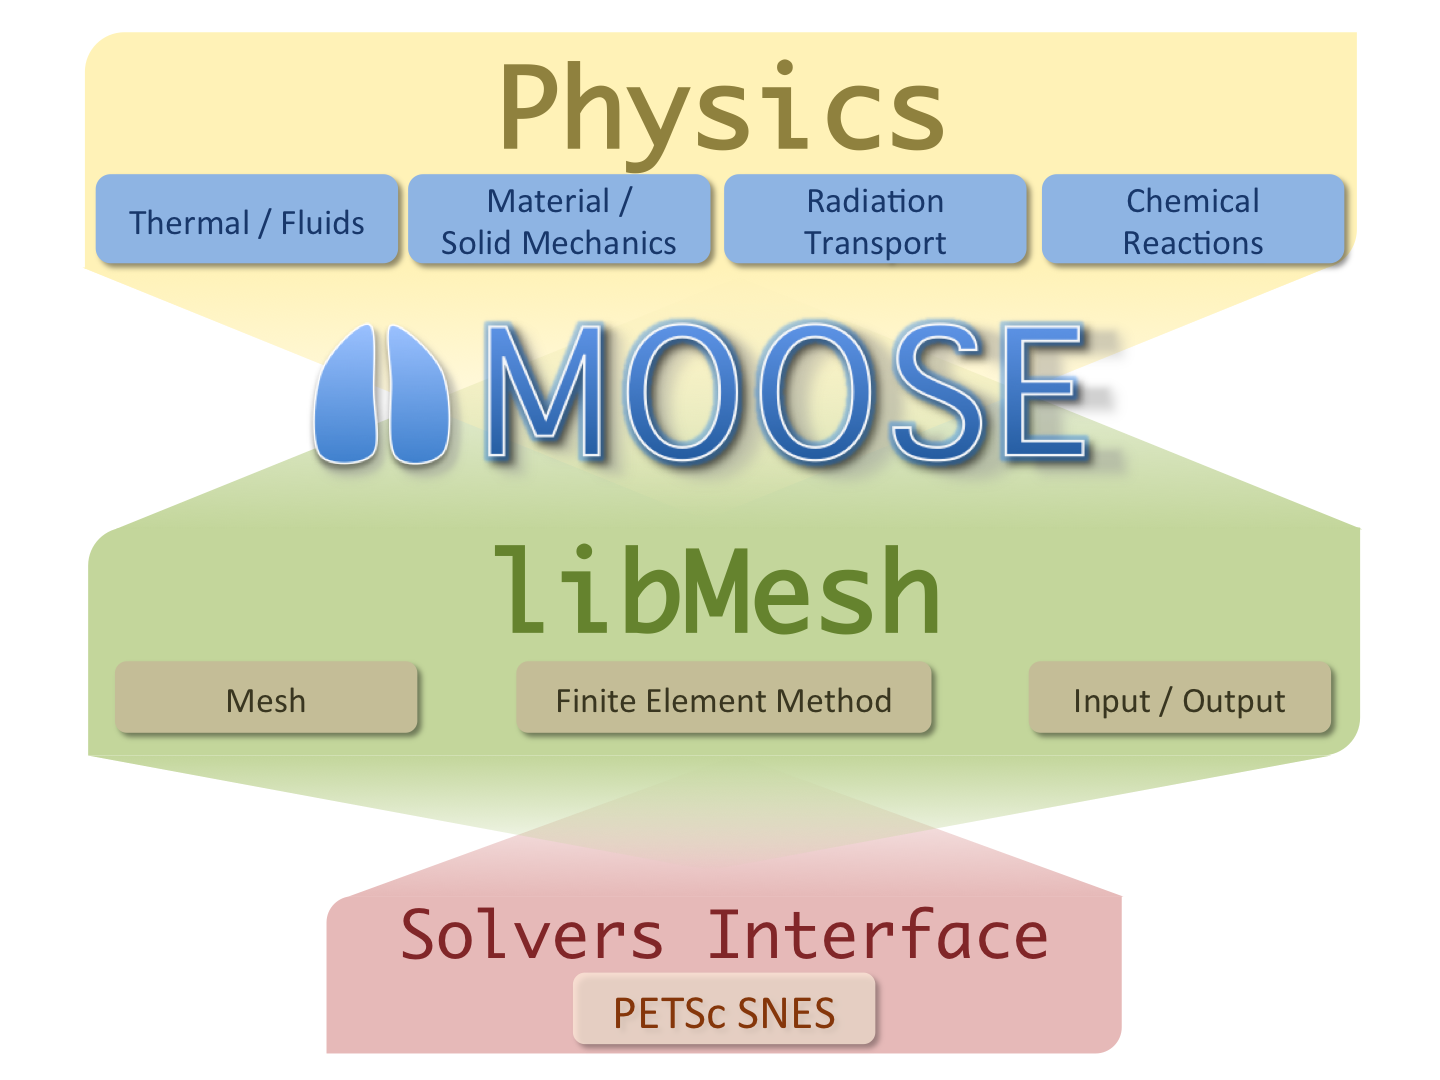
\includegraphics[width=0.65\textwidth]{figures/moose-arch} \\
  {\scriptsize \texttt{http://mooseframework.org/static/media/wiki/images/229/b61cdbc1e8be71dae37adc31a688d209/moose-arch.png}}
 \end{center}

\end{frame}


%%%%%%%%%%%%%%%%%

\begin{frame}{Providing Context}

 \begin{block}{Our Attempts in C++ Library Development}
  \begin{itemize}
   \item Sieve: Several years of C++ mesh management attempts in PETSc
   \item ViennaGrid 2.x: Heavily templated C++ mesh management library
   \item ViennaCL: Dense and sparse linear algebra and solvers for multi- and many-core architectures
  \end{itemize}
 \end{block}

 %\pause
 \begin{block}{Aftermath}
  \begin{itemize}
   \item Sieve: Replaced by DMPlex (written in C)
   \item ViennaGrid: Version 3.0 provides C-ABI
   \item ViennaCL: Rewrite in C likely
  \end{itemize}
 \end{block}

 \vspace*{-2cm}
 \begin{flushright}
  Sequential build times for the ViennaCL test suite \hspace*{0.2cm}\ \\
  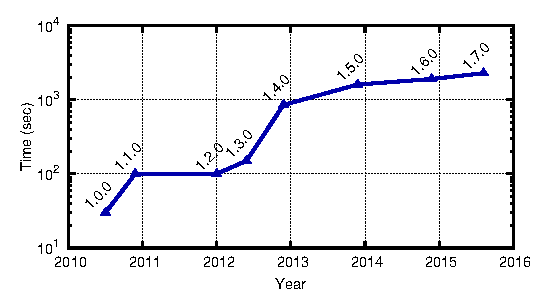
\includegraphics[width=0.55\textwidth]{figures/build-time}
 \end{flushright}

\end{frame}

%%%%%%%%%%%%%%%%%



\begin{frame}[fragile]{Disadvantages of C++ Templates}

 \begin{block}{Static Dispatch}
  \begin{itemize}
   \item Architecture-specific information only available at run time
   \item ``Change code and recompile'' not acceptable advice
  \end{itemize}
 \end{block}

 %\pause
 \begin{block}{Dealing with Compilation Errors}
  \begin{itemize}
   \item Type names pollute compiler output
   \item Replicated across interfaces
   \item CRTP may result in type length explosion
   \item Default arguments become visible \\[0.5em]
\begin{tabular}{|l|r|}
 \hline
  Type   & Length \\ 
 \hline
 \lstinline|std::vector<int>|                                           &  38 \\
 \lstinline|std::vector<std::vector<int> >|                             & 109 \\
 \lstinline|std::vector<std::vector<std::vector<int> > >|               & 251 \\
 \lstinline|std::vector<std::vector<std::vector<std::vector<int> > > >| & 539 \\
 \hline
\end{tabular}
  \end{itemize}
 \end{block}

 \vspace*{-7.5cm}
 \begin{flushright}
  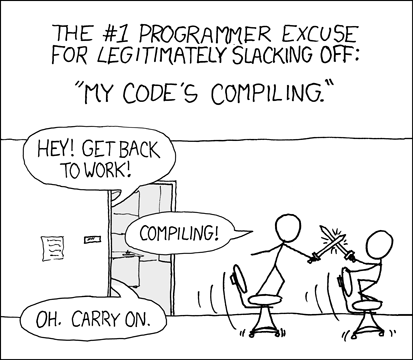
\includegraphics[width=0.35\textwidth]{figures/xkcd-compiling} \\
  {\scriptsize https://xkcd.com/303/}
 \end{flushright}
 \vspace*{2.5cm}

\end{frame}

%%%%%%%%%%%%%%%%%

\begin{frame}{Disadvantages of C++ Templates}

 \begin{center}
  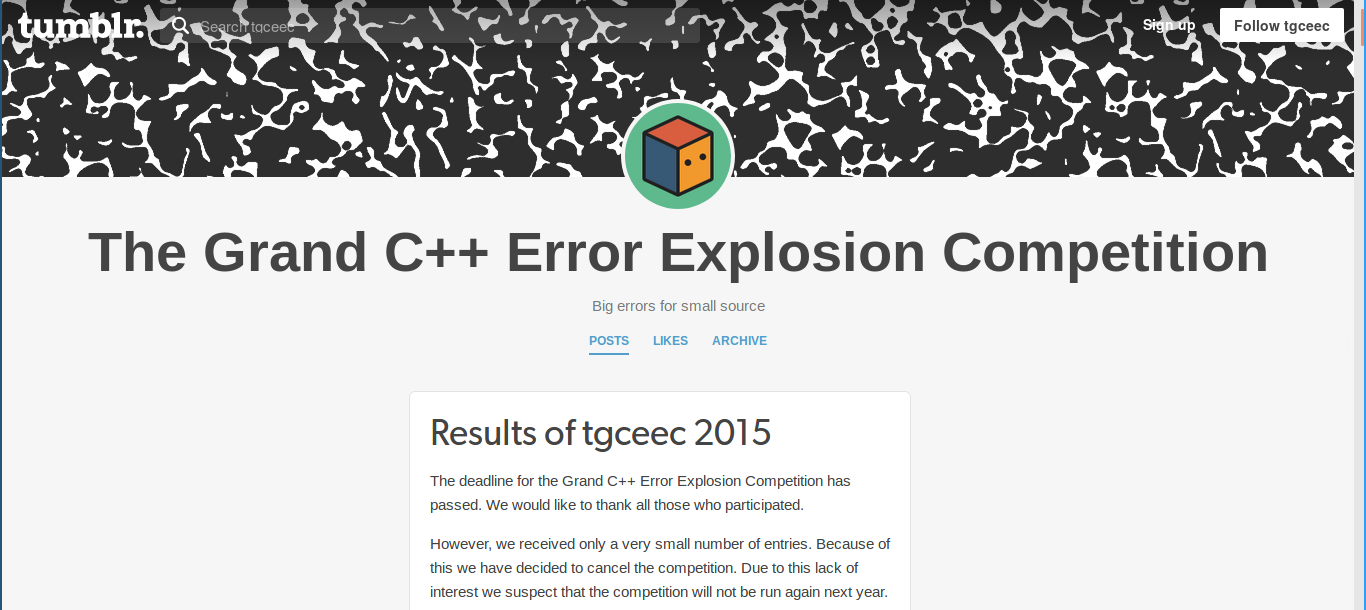
\includegraphics[width=0.95\textwidth]{figures/code-explosion} \\[0.5em]
  {\scriptsize \texttt{https://tgceec.tumblr.com/}}
 \end{center}

\end{frame}

%%%%%%%%%%%%%%%%%

\begin{frame}{Disadvantages of C++ Templates}

 \begin{block}{Scope Limitations}
  \begin{itemize}
   \item Template metaprogramming lacks state
   \item Optimizations across multiple code lines difficult or impossible
  \end{itemize}
 \end{block}

 %\pause
 \begin{block}{Example}
  \begin{itemize}
   \item Consider vector updates in pipelined CG method:
\begin{align*}
  x_i &\leftarrow x_{i-1} + \alpha  p_{i-1} \\
  r_i &\leftarrow r_{i-1} - \alpha  y_i \\
  p_i &\leftarrow r_i + \beta  p_{i-1}
\end{align*}
  \item Reuse of $p_{i-1}$ and $r_{i-1}$ easy with for-loops, but hard with expression templates

  \end{itemize}
 \end{block}

\end{frame}



%%%%%%%%%%%%%%%%%

\begin{frame}{Disadvantages of C++ Templates}

 \begin{block}{Complicates Debugging}
  \begin{itemize}
   \item Stack traces get longer names and deeper
   \item Setting good breakpoints may become harder
  \end{itemize}
 \end{block}

 %\pause
 \begin{block}{Lack of a Stable ABI}
  \begin{itemize}
   \item Object files from different compilers generally incompatible
   \item Name mangling makes use outside C++ land almost impossible
  \end{itemize}
 \end{block}

 %\pause
 \begin{block}{High Entry Bar}
  \begin{itemize}
   \item Number of potential contributors inversely proportional to code sophistication
   \item Domain scientists have limited resources for C++ templates
  \end{itemize}
 \end{block}


\end{frame}






%%%%%%%%%%%%%%%%%

\begin{frame}{A Path Forward}
 
 \begin{block}{Manage Complexity}
  \begin{itemize}
   \item Good interface design
   \item Refactor code when needed
   \item Hand-optimize small kernels only (cf.~BLIS methodology)
  \end{itemize}
 \end{block}
 
 \vspace*{-3.2cm}
 \begin{flushright}
  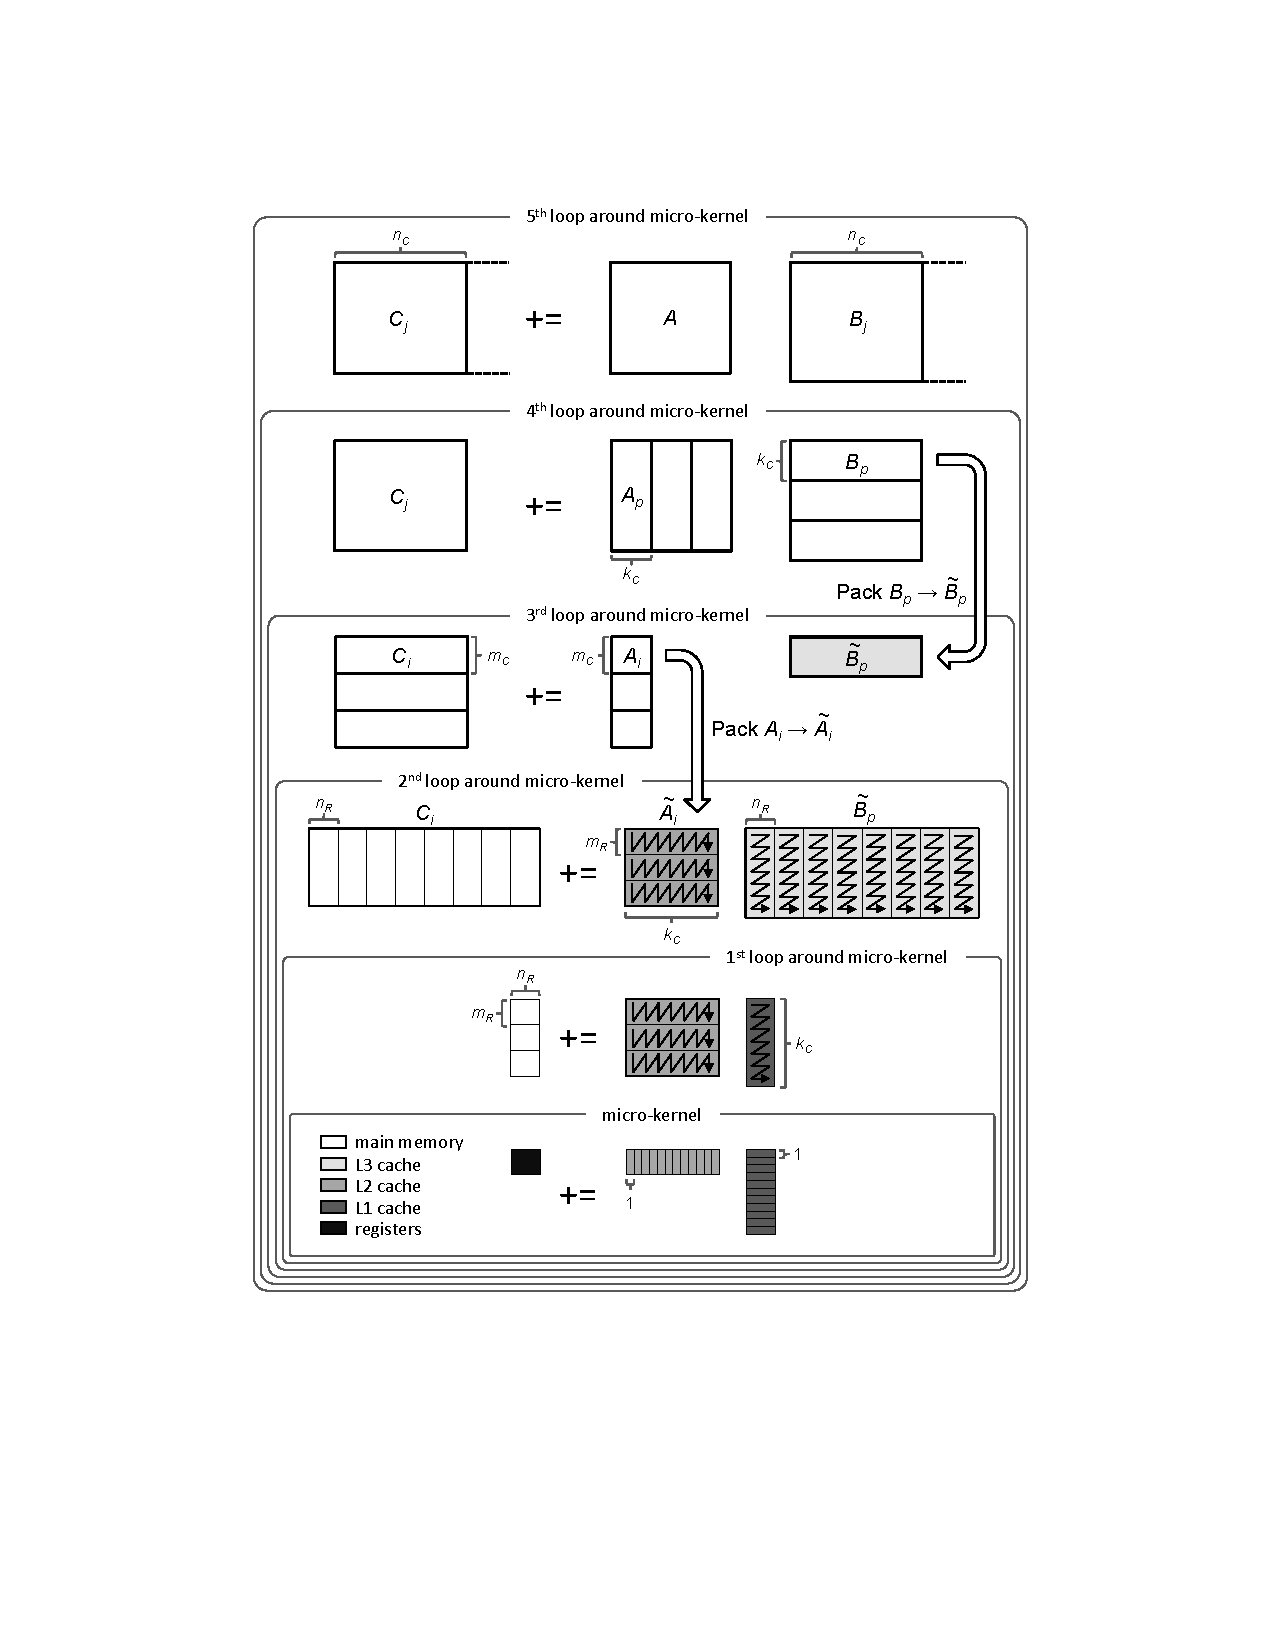
\includegraphics[width=0.36\textwidth]{figures/BLISLoops} \\
  {\scriptsize [F.~Van Zee, T.~Smith, ACM TOMS 2017]}
 \end{flushright}

 \vspace*{-4.5cm}
 %\pause
 \begin{block}{Development Implications}
  \begin{itemize}
   \item Adopt professional software development practices %(coding standards, rigorous testing, etc.)
   \item Develop, maintain, and evolve different datastructures ...
   \item ... and code paths
   \item Use clear and easy-to-understand datastructures
   \item Fallacy: ``Writing'' an application only once in its final form %and reusing it for decades is a fallacy
  \end{itemize}
 \end{block}
 
\end{frame}



%%%%%%%%%%%%%%%%%

\begin{frame}{A Path Forward}
 
 \begin{block}{Spending Development Resources}
  \begin{itemize}
   \item Reuse existing libraries --- reinventing the wheel is not productive!
   \item Focus on domain- and application-specific aspects
   \item Obtain expertise and resources for continuous code evolution
  \end{itemize}
 \end{block}

 %\pause
 \begin{block}{Required Incentives}
  \begin{itemize}
   \item Reward contributions to existing projects
   \item Pair research funding with software development funding
   \item Establish software development career tracks
  \end{itemize}
 \end{block}
 
\end{frame}


%%%%%%%%%%%%%%%%%

\begin{frame}{A Path Forward}
 
 \begin{block}{Is Performance Portability Just a Software Productivity Aspect?}
  \begin{center}
  \fbox{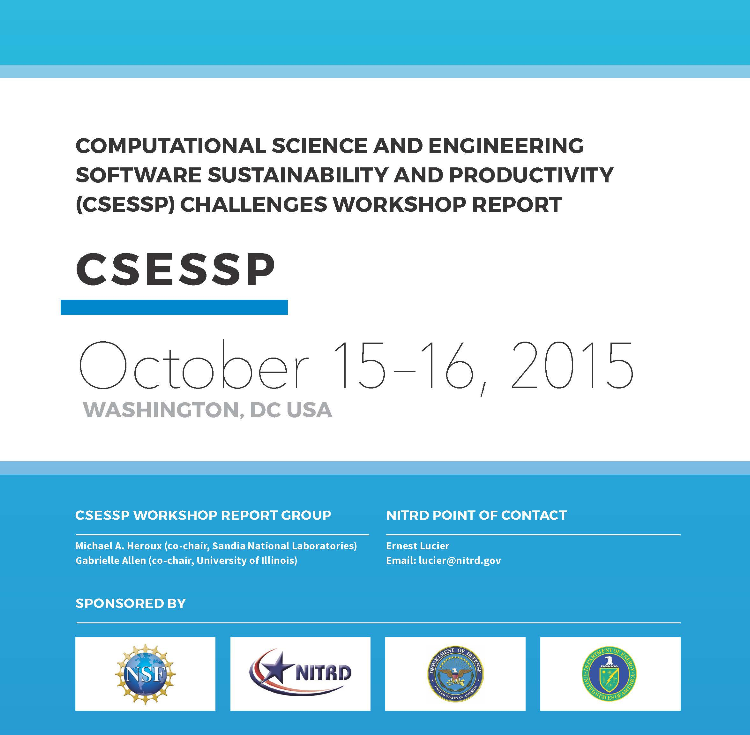
\includegraphics[width=0.4\textwidth]{figures/CSESSPWorkshopReport-front-page.png}} \\
  {\footnotesize \texttt{https://www.nitrd.gov/PUBS/CSESSPWorkshopReport.pdf}}
  \end{center}
 \end{block}
 
\end{frame}




\begin{frame}{Summary}

 \begin{block}{Long-Term Problems of Heavy C++ Templates Use}
  \begin{itemize}
   \item Template metaprogramming is a leaky abstraction
   \item Excessive type names slow down all stages of Compile-Run-Debug-cycle
   \item Templates operate at compile time - architecture ultimately known at run time
  \end{itemize}
 \end{block}
 
 \begin{block}{A Path Forward}
  \begin{itemize}
   \item Adopt professional software development practices
   \item Be prepared to develop different datastructures and code paths
   \item Write clear, readable code using simple datastructures
   \item Evolve and refactor datastructures, kernels, and interfaces over time
   \item \emph{(cf.~software productivity discussions)}
  \end{itemize}
 \end{block}
 

\end{frame}
